\chapter{天体辐射机制的量子语言}
\label{chap:e16}

\begin{chapteropening}
到这里为止，我们已经把一整套光的量子工具箱装配完毕：一个模式里平均有多少光子（第 \ref{chap:e05} 章的玻色占有数 \(\bar n_\nu\)），这些光子分布成什么样的量子态（第 \ref{chap:e06} 章的数态、相干态、热态），以及怎样用二阶相干函数 \(g^{(2)}\) 把不同的态区分开（第 \ref{chap:e08} 章）。现在我们第一次把望远镜真正对准天空。一颗恒星、一团 HII 区、一条喷流、一个 maser 斑、一个快速射电暴，它们最后都在探测器上留下一条 \(I_\nu\) 谱线；可它们背后的光场统计可以天差地别。本章是全书第 4 部分的开篇，任务只有一句话：把天体上五花八门的辐射机制，全部翻译成"模式占有数 + 光子统计"这一种语言，看清哪些机制天生给混沌热光、哪些可能偏离、以及为什么在天体上想抓到一束真正的非经典光会那么难。
\end{chapteropening}

\section{把辐射机制翻译成占有数和光子统计}
\label{sec:e16-translation}

辐射机制的传统入口是比强度（specific intensity）\(I_\nu\)，也就是单位时间、单位面积、单位频率、单位立体角内穿过的辐射能流，CGS 单位是 \({\rm erg\,s^{-1}\,cm^{-2}\,Hz^{-1}\,sr^{-1}}\)。若源在天空上张开的立体角是 \(\Omega_{\rm s}\)，望远镜收到的流量密度（flux density）近似为 \(S_\nu\simeq I_\nu\,\Omega_{\rm s}\)，常用单位 Jy（\(1~{\rm Jy}=10^{-23}~{\rm erg\,s^{-1}\,cm^{-2}\,Hz^{-1}}\)）。教科书讲辐射机制，往往到 \(I_\nu(\nu)\) 这条谱就停了。

问题是：谱只是一个"平均值"。你可以把同一条 \(I_\nu\) 谱，用完全不同的光场拼出来。想象两个池塘表面都起伏着高度相同的波纹——一个池塘的波纹是无数雨点各自砸出来、互不相干地叠加的；另一个池塘的波纹是有人在岸边有节奏地拍水、许多波峰步调一致推出来的。站得远远地量"平均起伏高度"，两个池塘一模一样；可只要你盯着水面看它\emph{涨落}的方式，两者立刻分道扬镳。天体辐射也是这样：平均谱 \(I_\nu\) 抹掉了光子到达时间的相关、偏振的相关、频率通道之间的联合概率——而这些，恰恰是辐射机制留下的指纹。

要把这些指纹量化，我们回收前面两章建立的两个相干函数。设 \(\hat E^{(+)}(t)\) 是正频电场算符（它对应"湮灭一个光子"，见第 \ref{chap:e05} 章），\(\hat E^{(-)}(t)=[\hat E^{(+)}(t)]^\dagger\)。归一化一阶相干函数为
\begin{equation}
  g^{(1)}(\tau)=
  \frac{\langle \hat E^{(-)}(t)\,\hat E^{(+)}(t+\tau)\rangle}
       {\langle \hat E^{(-)}(t)\,\hat E^{(+)}(t)\rangle},
  \label{eq:e16-g1}
\end{equation}
\begin{formulaexplain}
\(g^{(1)}(\tau)\) 是归一化一阶相干函数，无量纲。分子把 \(t\) 与 \(t+\tau\) 两个时刻的场关联起来，分母是平均强度。它衡量场的相位在延迟 \(\tau\) 后还记得多少，\(|g^{(1)}|\) 从 1（完全相干）降到 0（完全失忆）。
\end{formulaexplain}
分子 \(\langle \hat E^{(-)}(t)\hat E^{(+)}(t+\tau)\rangle\) 把两个时刻的场耦在一起，分母 \(\langle \hat E^{(-)}(t)\hat E^{(+)}(t)\rangle\) 就是平均强度，两者相除得到无量纲的量。\(|g^{(1)}(\tau)|\) 从 \(\tau=0\) 时的 1 衰减到大 \(\tau\) 时的 0，衰减的时间尺度就是相干时间 \(\tau_c\simeq1/\Delta\nu\)（第 \ref{chap:e02} 章）。它决定的是振幅干涉、谱线宽度、可见度这一层的物理。

二阶相干函数则问一个不同的问题——不是"相位还记得吗"，而是"一个光子到了，会不会带来另一个光子"：
\begin{equation}
  g^{(2)}(\tau)=
  \frac{\langle :\!\hat I(t)\,\hat I(t+\tau)\!:\rangle}{\langle \hat I(t)\rangle^2},
  \label{eq:e16-g2}
\end{equation}
\begin{formulaexplain}
\(g^{(2)}(\tau)\) 是归一化强度相关，无量纲；\(\hat I(t)\) 是瞬时强度算符，冒号表示正规序（把湮灭算符排到右边）。它比较两个时刻光子到达的联合概率与独立情形之比：\(>1\) 聚束，\(=1\) 泊松，\(<1\) 反聚束。
\end{formulaexplain}
这里 \(\hat I(t)\propto\hat E^{(-)}(t)\hat E^{(+)}(t)\) 是瞬时强度，冒号 \(:\ :\) 是正规序（normal ordering，把所有 \(\hat a^\dagger\) 排到 \(\hat a\) 左边，扣掉探测过程本身的散粒噪声，见第 \ref{chap:e08} 章）。\(g^{(2)}(\tau)\) 无量纲，它的物理是"条件概率"：给定 \(t\) 时刻探到一个光子，\(t+\tau\) 时刻探到另一个光子的概率，相对于两者独立时会高多少（\(>1\)，聚束 bunching）、一样（\(=1\)，泊松）、还是低（\(<1\)，反聚束 antibunching，只有非经典光才有）。

第 \ref{chap:e06} 与第 \ref{chap:e08} 章已经算清了三种参照态在 \(\tau=0\) 处的取值，我们把它当作已知结果点名在此：\emph{单模热（混沌）态} \(g^{(2)}(0)=2\)，\emph{相干态} \(g^{(2)}(0)=1\)，\emph{数态} \(g^{(2)}(0)<1\)。这就是本章的三把标尺。整章的核心工作，就是把每一种天体辐射机制放到这三把标尺之间：它默认落在哪一档？在什么条件下会偏离？以及——最关键的——真实观测会把它压到哪里去。

\section{亮温：把平均强度换算成占有数}
\label{sec:e16-brightness}

在动手翻译机制之前，我们需要一座桥，把观测直接量到的 \(I_\nu\) 换算成第 \ref{chap:e05} 章的模式占有数 \(\bar n_\nu\)。这座桥就是\emph{亮温}（brightness temperature）\(T_b\)。

在射电与远红外常用的 Rayleigh--Jeans（瑞利--金斯）形式里，把 \(I_\nu\) 反解成一个"等效温度"：
\begin{equation}
  T_b=\frac{c^2\,I_\nu}{2k_B\nu^2}
      =\frac{c^2\,S_\nu}{2k_B\nu^2\,\Omega_{\rm s}} .
  \label{eq:e16-brightness-temperature}
\end{equation}
\begin{formulaexplain}
\(T_b\) 是亮温，单位 K；\(c\) 光速，\(k_B\) Boltzmann 常数，\(\nu\) 频率，\(\Omega_{\rm s}\) 源立体角。它回答"若这点辐射在 R--J 极限下来自黑体，需要多高的温度"。它不是物质的真实温度。
\end{formulaexplain}
这里 \(c\) 是光速，\(k_B=1.38\times10^{-16}~{\rm erg\,K^{-1}}\) 是 Boltzmann 常数，\(\nu\) 是频率。\(T_b\) 的单位是 K，但请务必记住：它是一个\emph{定义}出来的等效量，回答的是"如果这份 \(I_\nu\) 来自 Rayleigh--Jeans 极限下的黑体，那黑体得多热"。对于非热电子、maser 或 FRB，\(T_b\) 完全不等于物质的热温度——它可以高到任何物理温度都望尘莫及。注意 \(T_b\propto S_\nu/\Omega_{\rm s}\)：源在天上越小，同样的流量密度推出来的 \(T_b\) 越高，所以角尺寸测量（VLBI）、变异时间尺度、散射展宽都会直接进到机制判断里。

现在把这座桥接到量子那一侧。一个偏振、一个频率模式的黑体比强度是 Planck 函数 \(B_\nu=(2h\nu^3/c^2)\,\bar n_\nu\)，其中占有数
\[
  \bar n_\nu=\frac{1}{\exp(h\nu/k_BT)-1}
\]
正是第 \ref{chap:e05} 章的主角。把这条式子里的 \(I_\nu=B_\nu\) 代进亮温定义 \eqref{eq:e16-brightness-temperature}，两边的 \(2\nu^2/c^2\) 约掉，直接得到一条极干净的对应关系：
\begin{equation}
  \bar n_\nu=\frac{k_B T_b}{h\nu}
  \qquad(\text{Rayleigh--Jeans 定义下，精确成立}).
  \label{eq:e16-occupation-from-tb}
\end{equation}
\begin{formulaexplain}
\(\bar n_\nu\) 是单个时空--偏振模式里的平均光子数；\(k_B T_b\) 是亮温对应的能量，\(h\nu\) 是单光子能量。这条式子说：\emph{亮温本质上就是占有数}，两者只差一个 \(h\nu/k_B\) 的换算。
\end{formulaexplain}
这一步是本章的"罗塞塔石碑"：\(\bar n_\nu=k_B T_b/(h\nu)\)。亮温不是别的，它就是模式占有数披了一件"温度"的外衣。\(T_b\) 高，等于每个模式里塞满了光子；\(T_b\) 低，等于模式几乎是空的。这一眼就把"平均谱"和"量子占有数"焊在了一起。

代两个真实数字进去，量级感立刻出来。其一，\emph{可见光下的恒星光球}：取 \(T\simeq6000~{\rm K}\)、\(\nu\simeq6\times10^{14}~{\rm Hz}\)（\(\lambda\simeq500~{\rm nm}\)），则 \(h\nu/k_BT=(6.6\times10^{-27}\times6\times10^{14})/(1.38\times10^{-16}\times6000)\simeq4.8\)，处在 Wien（维恩）区而不是 R--J 区，占有数 \(\bar n_\nu=1/(e^{4.8}-1)\simeq0.008\)。每个模式平均只有百分之一个光子！这解释了为什么恒星的可见光是一束极度"稀薄"的光，为什么 Hanbury Brown--Twiss 聚束信号那么微弱、为什么光子率在星际测量里是命门（第 \ref{chap:e10} 章）。其二，\emph{FRB}：一个毫秒、Jy 量级、Gpc 距离、GHz 频率的射电脉冲，代入 \eqref{eq:e16-brightness-temperature} 给出
\begin{equation}
  T_b\simeq
  1.1\times10^{35}~{\rm K}
  \left(\frac{S_\nu}{1~{\rm Jy}}\right)
  \left(\frac{D_A}{1~{\rm Gpc}}\right)^2
  \left(\frac{t_{\rm FRB}}{1~{\rm ms}}\right)^{-2}
  \left(\frac{\nu}{1~{\rm GHz}}\right)^{-2},
  \label{eq:e16-frb-tb}
\end{equation}
\begin{formulaexplain}
\(S_\nu\) 脉冲流量密度，\(D_A\) 角直径距离，\(t_{\rm FRB}\) 脉冲宽度，\(\nu\) 观测频率。这个天文数字说明毫秒 FRB 的亮温远超任何非相干辐射能达到的上限。
\end{formulaexplain}
其中 \(D_A\) 是角直径距离（脉冲宽度 \(t_{\rm FRB}\) 通过 \(\Omega_{\rm s}\lesssim(c\,t_{\rm FRB}/D_A)^2\) 的因果限制给出源尺度上限）。把 \(T_b\sim10^{35}~{\rm K}\)、\(\nu=1~{\rm GHz}\) 代入 \eqref{eq:e16-occupation-from-tb}：\(\bar n_\nu\simeq k_BT_b/(h\nu)=(1.38\times10^{-16}\times10^{35})/(6.6\times10^{-27}\times10^{9})\simeq2\times10^{36}\)。每个模式里挤着 \(10^{36}\) 个光子——这已经不是"许多独立粒子各自发光"能解释的了，它要求海量带电粒子在小于波长或相位可控的尺度上\emph{协同}发射 \citep{2007Sci...318..777L,2019A&ARv..27....4P,2022A&ARv..30....2P}。占有数在这里替我们喊出了"相干"两个字。

\begin{figure}[tbp]
\centering
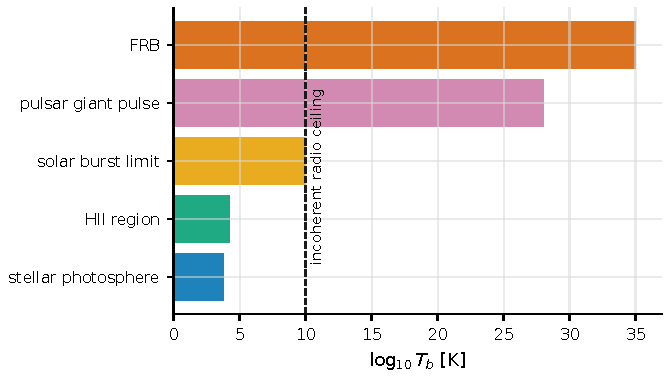
\includegraphics[width=0.82\linewidth]{figures/generated/chapter_09/ch09_brightness_temperature_scale.pdf}
\caption{亮温作为辐射机制的第一层判据。恒星光球和 HII 区落在普通热温度范围（对应占有数 \(\bar n_\nu\lesssim1\)）；太阳和恒星射电爆发若超过 \(10^{10}~{\rm K}\) 往往需要相干机制；脉冲星巨脉冲和 FRB 的亮温更高（占有数可达 \(10^{30}\) 以上），只能由相干发射或强束射几何解释。虚线标出常用的非相干射电上限量级。}
\label{fig:e16-brightness-temperature}
\end{figure}

亮温给我们的是一条硬的、经验性的门槛。Dulk 对太阳与恒星射电辐射的综述给出一条实用判据：非相干射电辐射的 \(T_b\) 很难超过 \(10^9\)--\(10^{10}~{\rm K}\)，这一上限主要来自回旋同步自吸收与能量学约束（占有数一旦太高，自吸收和辐射反作用就把它压回来；顺带一提，逆康普顿灾变 Kellermann--Pauliny-Toth 给出的是更高的 \(\sim10^{12}~{\rm K}\) 尺度，两者别混为一谈）；显著高于这个范围的爆发就必须请出相干机制，如等离子体辐射或 electron-cyclotron maser \citep{1985ARA&A..23..169D}。于是亮温标尺（图 \ref{fig:e16-brightness-temperature}）就成了机制判断的第一刀：占有数是 \(\lesssim1\) 的"稀薄热光"，还是 \(10^{20}\)、\(10^{30}\) 的"相干爆发"。但这只是第一刀——它只管平均能量密度合不合理，管不了这些光子是独立叠加还是协同发射。要分这一步，得动用光子统计。

\section{热辐射为什么天生是混沌光}
\label{sec:e16-thermal}

先看谱系里最"老实"的一档：热辐射。恒星光球、尘埃、HII 区、宇宙微波背景，都近似处在局部热平衡（local thermodynamic equilibrium）。它们的模式占有数由 Planck 分布给出，
\begin{equation}
  \bar n_\nu=\frac{1}{\exp(h\nu/k_BT)-1},
  \label{eq:e16-planck-occupation}
\end{equation}
\begin{formulaexplain}
\(\bar n_\nu\) 频率 \(\nu\) 模式的平均占有数；\(h\nu\) 单光子能量，\(T\) 物质温度。R--J 区（\(h\nu\ll k_BT\)）\(\bar n_\nu\approx k_BT/h\nu\gg1\)；Wien 区（\(h\nu\gg k_BT\)）\(\bar n_\nu\approx e^{-h\nu/k_BT}\ll1\)。
\end{formulaexplain}
这里 \(T\) 是物质的热温度。注意恒星光球的可见光常处在 Wien 区（\(h\nu/k_BT>1\)），所以颜色温度、有效温度、亮温三者不能混用——同一颗星，射电端 \(\bar n_\nu\) 大、光学端 \(\bar n_\nu\) 小。但无论落在哪个区，热态的\emph{统计性质}都一样，而这正是我们关心的。

为什么热辐射天生给混沌光（chaotic light）？物理图像是这样的：热光源里有海量独立的发射体（原子、离子、电子），每一个都在随机的时刻、以随机的相位发出一个小波列。探测器接到的总电场，是这千千万万个相位随机、幅度随机的小箭头的矢量和。这时候中心极限定理（central limit theorem）登场——大量独立随机量之和趋向高斯分布——所以窄带内的复电场 \(\hat E^{(+)}(t)\) 是一个\emph{复高斯随机过程}（complex Gaussian random process）。这不是巧合，是"许多独立事件相加"的必然结果。

高斯随机过程有一个漂亮的代数性质（第 \ref{chap:e08} 章证过，这里点名为已知结果）：它的四阶矩可以拆成二阶矩的乘积（矩定理 / Gaussian moment theorem）。把这条性质用到 \eqref{eq:e16-g2} 的分子上，就得到 Siegert（西格特）关系
\begin{equation}
  g^{(2)}(\tau)=1+\frac{|g^{(1)}(\tau)|^2}{M_{\rm eff}},
  \label{eq:e16-siegert}
\end{equation}
\begin{formulaexplain}
Siegert 关系：混沌（高斯）光的二阶相干完全由一阶相干决定。\(M_{\rm eff}\) 是被同时平均的模式数。单模（\(M_{\rm eff}=1\)、\(\tau=0\)）给出 \(g^{(2)}(0)=1+1=2\)，就是热光聚束峰。
\end{formulaexplain}
在单一时空--偏振模式里（\(M_{\rm eff}=1\)）取 \(\tau=0\)，因为 \(|g^{(1)}(0)|=1\)，立刻得到 \(g^{(2)}(0)=1+1=2\)。这就是热光聚束的种子，也是本章反复要用的锚点：\emph{只要是"许多独立发射体相加"，光场就是高斯混沌场，就自带 \(g^{(2)}(0)=2\) 的聚束峰。}热光并不神秘，它的聚束纯粹是相位随机叠加时"强度会成团涨落"的统计后果。

这个逻辑的力量在于它\emph{不挑机制}。只要满足"许多独立事件相加、窄带内相位随机"，谱形是什么无所谓，结论都是高斯混沌光。第一个例子是\emph{自由自由辐射}（bremsstrahlung，轫致辐射）：它不是黑体谱本身，而是无数电子在离子库仑场中被加速、各自发一次刹车辐射的连续谱。单次碰撞的相位完全不可预测，窄带内的复电场照样趋向高斯过程。稀薄电离气体中，发射系数的量级为
\begin{equation}
  j_\nu^{\rm ff}\propto
  n_e\,n_i\,T_e^{-1/2}
  \exp\!\left(-\frac{h\nu}{k_BT_e}\right)
  g_{\rm ff}(\nu,T_e),
  \label{eq:e16-free-free}
\end{equation}
\begin{formulaexplain}
\(j_\nu^{\rm ff}\) 自由自由发射系数；\(n_e,n_i\) 电子、离子数密度（\({\rm cm^{-3}}\)），\(T_e\) 电子温度，\(g_{\rm ff}\) Gaunt 因子（\(\sim1\) 到数十）。它是许多独立库仑碰撞贡献的连续谱。
\end{formulaexplain}
其中 \(n_e,n_i\) 是电子和离子数密度（\({\rm cm^{-3}}\)），\(T_e\) 是电子温度，\(g_{\rm ff}\) 是 Gaunt 因子。HII 区的 \(T_e\sim10^4~{\rm K}\)，星风、吸积流可以更高。谱形（射电端近平坦、高频指数衰减）和黑体完全不同，但光子统计一样是混沌热光，同样自带 \(g^{(2)}(0)=2\) 的种子。

不过谱要观测到，还得穿过介质，这就要放进辐射转移方程（radiative transfer equation）：
\begin{equation}
  \frac{{\rm d}I_\nu}{{\rm d}s}=j_\nu-\alpha_\nu I_\nu,
  \qquad
  S_\nu=\frac{j_\nu}{\alpha_\nu}.
  \label{eq:e16-radiative-transfer}
\end{equation}
\begin{formulaexplain}
\({\rm d}I_\nu/{\rm d}s\) 沿视线的强度变化；\(j_\nu\) 加入辐射，\(\alpha_\nu I_\nu\) 吸收辐射，\(S_\nu=j_\nu/\alpha_\nu\) 源函数。它把发射机制和光深连起来。
\end{formulaexplain}
\(s\) 是沿视线距离，\(j_\nu\) 是发射系数，\(\alpha_\nu\) 是吸收系数，源函数 \(S_\nu=j_\nu/\alpha_\nu\)。定义光深 \({\rm d}\tau_\nu=\alpha_\nu\,{\rm d}s\)，把 \eqref{eq:e16-radiative-transfer} 对一块均匀 slab 积分（这是一阶线性常微分方程，用积分因子 \(e^{\tau_\nu}\) 直接解，标准结果），再换成亮温，得到
\begin{equation}
  T_b=T_{\rm eff}\left(1-e^{-\tau_\nu}\right)+T_{\rm bg}\,e^{-\tau_\nu}.
  \label{eq:e16-tb-transfer}
\end{equation}
\begin{formulaexplain}
\(T_b\) 出射亮温；\(T_{\rm eff}\) 源函数对应温度，\(T_{\rm bg}\) 背景亮温，\(\tau_\nu\) 光深。薄源（\(\tau_\nu\ll1\)）只加一点点，厚源（\(\tau_\nu\gg1\)）趋向自身源函数。
\end{formulaexplain}
光深很小时 \(T_b\simeq T_{\rm eff}\tau_\nu+T_{\rm bg}\)（薄源只贡献小增量），光深很大时 \(T_b\to T_{\rm eff}\)（厚源热化到自身源函数）。这条式子常用来判断一个源是热化的、半透明的、还是非热占优的 \citep{1979rpa..book.....R,2011piim.book.....D,1985ARA&A..23..169D}。它也解释了亮温上限从何而来：一旦光深足够大，\(T_b\) 就被源函数（对热源就是物质温度）卡死，涨不上去。

小结这一节的物理：热辐射与自由自由辐射的共同点，不在谱形，而在"许多独立发射体相加"这条统计根。这条根让它们的电场都是高斯混沌场，都默认坐在 \(g^{(2)}(0)=2\) 那一档。这就是我们的"零点"——接下来所有其他机制，都要看它们是留在这一档、还是偏离。

\section{非热粒子：谱和偏振变了，统计却常常没变}
\label{sec:e16-nonthermal}

初学者最容易犯的一个错，是把"非热"（non-thermal）和"非高斯统计"划等号。这一节要专门破除它。同步辐射、逆康普顿——它们的\emph{谱和偏振}确实彻底偏离黑体，但它们的\emph{光子统计}多半仍然是高斯混沌光。原因还是那条根：只要发光的是许多独立粒子、窄带内相位随机，中心极限定理照样把电场压成高斯过程。

同步辐射（synchrotron radiation）来自相对论电子在磁场中的螺旋运动。单个电子的特征频率是
\begin{equation}
  \nu_c=\frac{3eB\sin\alpha}{4\pi m_ec}\,\gamma^2 ,
  \label{eq:e16-synch-critical}
\end{equation}
\begin{formulaexplain}
\(\nu_c\) 同步特征频率；\(e\) 元电荷，\(B\) 磁场，\(\alpha\) 投掷角（pitch angle），\(m_e\) 电子质量，\(\gamma\) Lorentz 因子。频率随 \(B\) 和 \(\gamma^2\) 增长，所以高能电子能把辐射推到很高频段。
\end{formulaexplain}
其中 \(e\) 是元电荷，\(B\) 磁场强度，\(\alpha\) 投掷角，\(m_e\) 电子质量，\(\gamma\) Lorentz 因子。提醒一句：这里的裸符号 \(\alpha\) 专指投掷角（pitch angle，电子速度与磁场的夹角），请勿与上一节的吸收系数 \(\alpha_\nu\)、下文将出现的同步谱指数 \(\alpha_{\rm syn}\) 混淆——三者靠语境和下标区分。代数字：\(B=1~{\rm G}\)、\(\gamma=10^3\)、\(\sin\alpha=1\)，得 \(\nu_c\simeq4.2\times10^{12}~{\rm Hz}\)（远红外）；换到星系际或喷流尺度的弱磁场 \(B=10^{-5}~{\rm G}\)，同一批电子主要辐射在射电。真实源的发射系数是所有能量电子的贡献叠加，
\begin{equation}
  j_\nu^{\rm syn}=\int P_\nu(E,B,\alpha)\,N(E)\,{\rm d}E ,
  \label{eq:e16-synch-emissivity}
\end{equation}
\begin{formulaexplain}
\(j_\nu^{\rm syn}\) 同步发射系数；\(P_\nu\) 单电子功率谱，\(N(E)\) 电子能量分布。积分说明观测谱是所有能量电子贡献之和——正是"许多独立发射体相加"。
\end{formulaexplain}
若电子能谱是幂律 \(N(E)\propto E^{-p}\)，光薄同步辐射给出幂律谱 \(I_\nu\propto\nu^{-\alpha_{\rm syn}}\)，谱指数 \(\alpha_{\rm syn}=(p-1)/2\)。同步辐射的招牌是高线偏振——均匀磁场里最大线偏振度为
\begin{equation}
  \Pi_{\rm syn}=\frac{p+1}{p+7/3}.
  \label{eq:e16-synch-polarization}
\end{equation}
\begin{formulaexplain}
\(\Pi_{\rm syn}\) 光薄同步辐射最大线偏振度；\(p\) 电子能谱指数。它是均匀磁场加幂律电子分布下偏振的理论上限。
\end{formulaexplain}
例如 \(p=2.4\) 时 \(\Pi_{\rm syn}\simeq72\%\)。实际喷流、超新星遗迹、脉冲星风云的偏振往往低得多，因为磁场方向杂乱、法拉第旋转、束内平均、多发射区叠加都会抵消偏振。请注意关键的一点：式 \eqref{eq:e16-synch-emissivity} 的积分号本身就在说"许多独立电子相加"，所以\emph{尽管谱是幂律、偏振很高，电场依然近似高斯混沌场，\(g^{(2)}(0)\) 依然默认是 2}。同步辐射改写的是平均谱和偏振（由非热电子分布和磁场几何决定），没改写光子统计这一档 \citep{1965ARA&A...3..297G,1970RvMP...42..237B,1978bllo.conf..328B,2012ApJ...752..157Z}。

逆康普顿散射（inverse Compton scattering）把低能种子光子踢到高能。Thomson 极限下，散射后光子能量的量级是
\begin{equation}
  h\nu_{\rm IC}\sim\gamma^2\,h\nu_{\rm seed}.
  \label{eq:e16-ic-energy}
\end{equation}
\begin{formulaexplain}
\(h\nu_{\rm seed}\) 种子光子能量，\(h\nu_{\rm IC}\) 散射后能量，\(\gamma\) 电子 Lorentz 因子。Thomson 极限中一次散射把光子能量提升约 \(\gamma^2\) 倍。
\end{formulaexplain}
热电子云中的多次散射，用 Compton \(y\) 参数衡量：
\begin{equation}
  y\simeq4\,\frac{k_BT_e}{m_ec^2}\,\max(\tau_T,\tau_T^2),
  \label{eq:e16-compton-y}
\end{equation}
\begin{formulaexplain}
\(y\) Comptonization 强度参数；前因子 \(4k_BT_e/m_ec^2\) 是单次散射的相对能量增益，\(\max(\tau_T,\tau_T^2)\) 估平均散射次数（\(\tau_T\) Thomson 光深）。它判断谱被电子云改写到什么程度。
\end{formulaexplain}
\(y\ll1\) 谱只被轻微改动；\(y\sim1\) 形成明显的 Comptonized 连续谱；\(y\gg1\) 趋向饱和 Comptonization。在 X 射线双星、AGN 冕（corona）、GRB 光球模型里，平均谱常由同步、热光子、逆康普顿几个分量混出来，单看谱指数几乎无法唯一定机制 \citep{1980A&A....86..121S,1999MNRAS.309..496G,2013ApJ...765..103L}。而这些散射过程涉及的仍是海量独立光子--电子事件，输出光场的统计还是留在混沌热光那一档。

\begin{figure}[tbp]
\centering
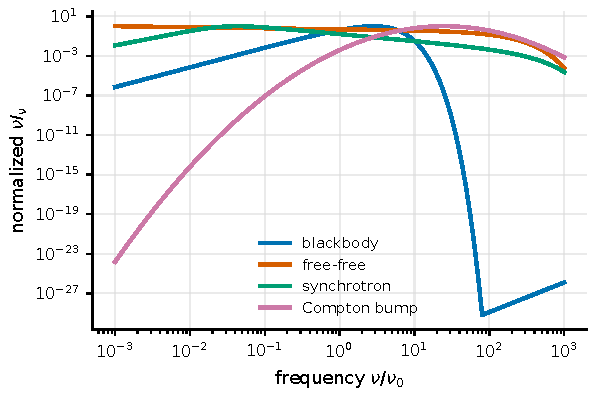
\includegraphics[width=0.84\linewidth]{figures/generated/chapter_09/ch09_spectral_mechanisms.pdf}
\caption{常见连续辐射机制的归一化谱形示意。黑体有热峰和 R--J 低频端；自由自由辐射在射电近平坦、高频指数衰减；同步辐射由非热电子能谱给出幂律加高低频截断；逆康普顿分量常表现为高能鼓包。四种谱形迥异，但只要是"许多独立粒子相加"，光子统计都默认落在 \(g^{(2)}(0)=2\) 的混沌热光那一档。}
\label{fig:e16-spectral-mechanisms}
\end{figure}

这一节的教学要点，一句话：\emph{谱和偏振能告诉你粒子分布和磁场几何，但告诉不了你光子统计。}热的、自由自由的、同步的、逆康普顿的——谱形从热峰到幂律到高能鼓包一路变化（图 \ref{fig:e16-spectral-mechanisms}），可它们共享同一条统计根，都是高斯混沌光。要让 \(g^{(2)}\) 真正偏离 2，必须打破"许多独立发射体相加"这个前提——这就把我们逼到下一节的相干机制。

\section{相干机制：突破亮温上限的少数出口}
\label{sec:e16-coherent}

要偏离混沌热光，只有一条路：让发射体不再独立，让大量电荷在相位上\emph{协同}起来。一旦协同，中心极限定理的前提就垮了，电场不再是高斯过程，占有数可以冲上 \(10^{20}\)、\(10^{30}\)，亮温突破那条 \(10^{10}~{\rm K}\) 的非相干上限。天体上做到这一点的机制屈指可数，本节逐个点名。

\paragraph{受激辐射类：maser 与激光}
\label{sec:e16-maser}

Maser（微波激射）从"负吸收"开始。若某条谱线上出现粒子数反转（population inversion，高能级比低能级还多），吸收系数就变成负的，\(\alpha_\nu<0\)。把它代进辐射转移，强度沿路径\emph{指数放大}：
\begin{equation}
  I_\nu(L)\simeq I_\nu(0)\,\exp(|\tau_m|),
  \qquad
  \tau_m=\int_0^L\alpha_\nu\,{\rm d}s<0 .
  \label{eq:e16-maser-gain}
\end{equation}
\begin{formulaexplain}
\(I_\nu(0),I_\nu(L)\) 路径前后强度；\(\tau_m<0\) 负吸收光深。未饱和时增益随 \(|\tau_m|\) 指数增长——这是高亮温窄线的来源。
\end{formulaexplain}
未饱和时增益对光深指数敏感，能把 \(T_b\) 推到极高；饱和后受激辐射耗尽反转，线宽、偏振、强度都由泵浦和几何接管。水 maser、OH maser、SiO maser 的亮温可以极高，占有数因而巨大。但要小心：天体 maser 的相干性通常由许多速度相干路径、湍动团块、偏振传播效应共同决定，\emph{不能}简单等同于实验室里那束单模激光的近相干态。Goldreich、Keeley、Kwan 与 Elitzur 的工作给出了源尺寸、饱和、线宽、偏振的基本约束 \citep{1972ApJ...174..517G,1973ApJ...179..111G,1974ApJ...190...27G,1982RvMP...54.1225E,1992ARA&A..30...75E}。受激辐射也不限于射电——Eta Carinae 的 Weigelt blobs 里，Fe II、O I 谱线在特定泵浦和光深下可出现激光或激光样放大，其线宽、位置、偏振和光子相关能检验反转与反馈几何 \citep{2004A&A...428..497J,2005NewA...10..361J,2008AIPC..984..216D}。只要泵浦、能级结构、逃逸路径合适，光学谱线也能带上非普通热光的统计特征。

电子回旋 maser（electron-cyclotron maser）是强磁化、低密度等离子体里的相干射电机制。它要求电子分布偏离平衡（如 loss-cone 分布），且回旋频率与等离子体频率的关系允许电磁波逃逸。回旋频率为
\begin{equation}
  \nu_B=\frac{eB}{2\pi m_ec}
       \simeq2.8~{\rm MHz}\left(\frac{B}{1~{\rm G}}\right).
  \label{eq:e16-cyclotron-frequency}
\end{equation}
\begin{formulaexplain}
\(\nu_B\) 电子回旋频率；\(e\) 电荷，\(B\) 磁场，\(m_e\) 电子质量。观测到的 maser 频率可反推发射区磁场量级。
\end{formulaexplain}
若在 GHz 频率看到基频或低次谐波的 electron-cyclotron maser，磁场量级就是几百 G 到几 kG。太阳、行星、褐矮星、低质量恒星的高圆偏振射电爆发都可落进这个框架 \citep{1982ApJ...259..844M,2006A&ARv..13..229T,2008ApJ...684..644H,1985ARA&A..23..169D}。

\paragraph{天线类：相干曲率辐射}
\label{sec:e16-curvature}

曲率辐射（curvature radiation）展示了通往相干性的另一条路——它不靠能级反转，而是让许多电荷在相位上协同运动，像一根天线。相对论电荷沿弯曲磁力线运动时，单个电荷的特征频率和功率为
\begin{equation}
  \nu_{\rm curv}=\frac{3c}{4\pi\rho}\gamma^3,
  \qquad
  P_{\rm curv}=\frac{2e^2c}{3\rho^2}\gamma^4 ,
  \label{eq:e16-curvature}
\end{equation}
\begin{formulaexplain}
\(\nu_{\rm curv}\) 曲率辐射特征频率，\(P_{\rm curv}\) 单粒子功率；\(\rho\) 磁力线曲率半径，\(\gamma\) Lorentz 因子。相干曲率辐射还需许多电荷相位同步。
\end{formulaexplain}
其中 \(\rho\) 是磁力线曲率半径。代数字：\(\rho=10^7~{\rm cm}\)、\(\gamma=300\)，先算前因子 \(3c/(4\pi\rho)\simeq7.2\times10^2~{\rm Hz}\)，再乘 \(\gamma^3=2.7\times10^7\)，得 \(\nu_{\rm curv}\sim2\times10^{10}~{\rm Hz}\)（仍属射电／微波波段）。单个粒子的曲率辐射太弱；相干曲率辐射要求许多电荷在小于波长的纵向尺度上成团（bunching），电场振幅\emph{相加}而非功率相加，于是总功率近似随粒子数\emph{平方}增长。这就是"天线"的精髓：\(N\) 个电荷若相位同步，辐射功率 \(\propto N^2\) 而非 \(N\)。这个思路长期用于脉冲星相干射电，也被搬进 FRB 模型 \citep{1977ApJ...212..800C,2018MNRAS.477.2470L}。

FRB 把相干机制推到极端。Lorimer burst 给出了毫秒时标、冷等离子体色散、\(T_b\sim10^{34}~{\rm K}\) 的第一组证据；重复源和 CHIME 样本显示重复、偏振、频率漂移、微结构、宿主环境都进模型；SGR 1935+2154 的 2020 年事件把银河系 magnetar 和 FRB 样射电暴直接连上了 \citep{2007Sci...318..777L,2019A&ARv..27....4P,2022A&ARv..30....2P,2020Natur.587...54C,2020Natur.587...59B}。众多模型大致两类：靠粒子数反转或激波的 maser 类，和靠电荷团块或电流片的天线/曲率类。微秒以下结构、强偏振、频率漂移、多波段非探测共同约束发射半径、Lorentz 因子、等离子体密度和辐射效率。

这一节的物理落点：相干机制之所以能突破亮温上限、把占有数推到天文数字，是因为它们打破了"独立发射体相加"这个前提，让电荷协同起来。它们的光子统计\emph{原则上}可以偏离混沌热光——但请记住，这里说的偏离，指的是极高占有数下受激/协同发射的特征，并不等于我们在实验室里追求的那种压缩态、反聚束的非经典光。真正的非经典光需要 \(g^{(2)}(0)<1\)，而天体上，哪怕源本身偏离了热统计，我们能不能\emph{测到}这份偏离，还要过下一节这一关。

\section{为什么天体上极难隔离真正的非经典光}
\label{sec:e16-dilution}

现在到了本章最要紧、也最容易被浪漫化的一点。前面说单模热光 \(g^{(2)}(0)=2\)，相干机制可能偏离——听上去只要架好探测器就能读出机制指纹。真实观测却几乎总是把这些指纹\emph{抹平}。抹平它的，是"模式稀释"（mode dilution）。

物理图像：\(g^{(2)}(0)=2\) 的那个漂亮聚束峰，只在\emph{单一}时空--偏振模式里成立。可真实望远镜同时收进一大堆模式——望远镜的接收面覆盖许多空间相干斑（空间模式 \(M_{\rm sp}\)），它对两个偏振都敏感（偏振模式 \(M_{\rm pol}\)），它的时间分辨率 \(\Delta t\) 又远宽于相干时间 \(\tau_c\)（时间模式 \(\sim\Delta t/\tau_c\)）。这些模式的涨落彼此独立，一平均，聚束峰就被摊薄。把 Siegert 关系 \eqref{eq:e16-siegert} 里的 \(M_{\rm eff}\) 写细，
\begin{equation}
  g^{(2)}_{\rm meas}(0)-1\simeq\frac{1}{M_{\rm eff}},
  \qquad
  M_{\rm eff}\simeq M_{\rm sp}\,M_{\rm pol}\left(1+\frac{\Delta t}{\tau_c}\right).
  \label{eq:e16-mode-dilution}
\end{equation}
\begin{formulaexplain}
\(M_{\rm eff}\) 有效混合模式数；\(M_{\rm sp},M_{\rm pol}\) 空间、偏振模式数，\(\Delta t/\tau_c\) 时间 bin 对相干时间的平均。模式越多，能测到的聚束对比度 \(g^{(2)}_{\rm meas}(0)-1\) 越低。
\end{formulaexplain}
其中 \(M_{\rm sp}\) 是被混合的空间模式数，\(M_{\rm pol}\) 是偏振模式数，\(\Delta t\) 是电子学或软件时间 bin，\(\tau_c\simeq1/\Delta\nu\) 是由光谱带宽决定的相干时间。代真实数字：可见光 \(\lambda=500~{\rm nm}\)、谱带宽 \(\Delta\lambda\simeq1~{\rm nm}\)（这里的 nm 是波长单位，标的是 \(\Delta\lambda\) 而非频率带宽），用 \(\Delta\nu\simeq c\,\Delta\lambda/\lambda^2\approx1.2\times10^{12}~{\rm Hz}\) 换成频率带宽，对应的相干时间约 \(\tau_c\simeq1/\Delta\nu\sim0.8~{\rm ps}\)；而典型电子学时间分辨率 \(\Delta t\sim100~{\rm ps}\)，于是 \(\Delta t/\tau_c\sim125\)。哪怕只有一个空间、一个偏振模式，单模热光本该到 2 的聚束峰，被压到 \(g^{(2)}_{\rm meas}(0)-1\sim1/125\lesssim0.01\)——足足两个数量级（图 \ref{fig:e16-mode-dilution}）。这就是为什么 Hanbury Brown--Twiss 强度干涉在星际尺度上信号那么微弱，为什么每一分对比度都要用窄带滤波、偏振选择、空间模式控制去"抢"，而每一步抢救对比度都以牺牲光子率为代价（第 \ref{chap:e10} 章会把这笔账算清）。

\begin{figure}[tbp]
\centering
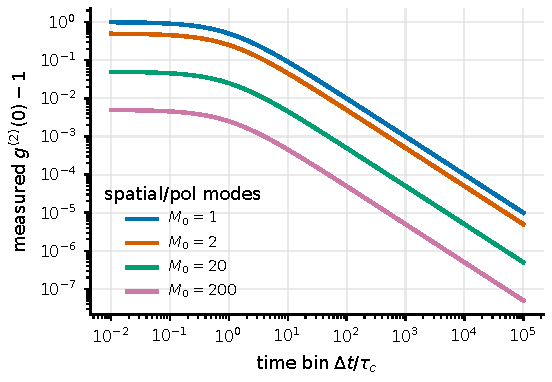
\includegraphics[width=0.82\linewidth]{figures/generated/chapter_09/ch09_thermal_mode_dilution.pdf}
\caption{热光聚束对比度随有效模式数下降。横轴是时间 bin 与相干时间之比，曲线上的 \(M_0\) 代表进入同一个相关估计器的空间与偏振模式数。即便源本身是纯热光，宽时间 bin、多偏振混合、多空间模式混合都会把 \(g^{(2)}(0)-1\) 拉向零——这正是天体上极难看到光子统计指纹的根本原因。}
\label{fig:e16-mode-dilution}
\end{figure}

现在把这层稀释叠到前面的图景上，就明白"天体上为什么极难隔离真正的非经典光"了。第一，多数机制\emph{本来}就给混沌热光（\(g^{(2)}(0)=2\)），非经典（\(g^{(2)}(0)<1\)）的候选屈指可数。第二，即便某个相干机制原则上偏离了热统计，模式稀释也会把可测的偏离压到 \(10^{-2}\) 甚至更低。第三，就算你信号还在，仪器和传播效应会伪造出假的相关：死时间、afterpulsing、时间戳量化、触发选择会改写到达时间相关（假的 \(g^{(2)}\) 结构）；等离子体闪烁、散射尾、引力微透镜、频率依赖吸收会造出跨频相关；热背景叠一条窄 maser 线、或同步连续谱叠一个相干脉冲，会让平均谱看着平滑、光子统计却不再单一。所以任何一个"反常的 \(g^{(2)}\) 峰"，都必须先和仪器、传播、混合源逐项对账，才敢往"非经典"上想（图 \ref{fig:e16-g2-diagnostics} 把单模热光、多模稀释、相干态、窄相干线四种情形的 \(g^{(2)}(\tau)\) 形状放在一起对照，正是这一步逐项排查的参照图）。第 \ref{chap:e13} 章和第 \ref{chap:e14} 章的事件表、时间移位背景、协方差估计，提供的正是这种逐项排查所需的分析层。

\begin{figure}[tbp]
\centering
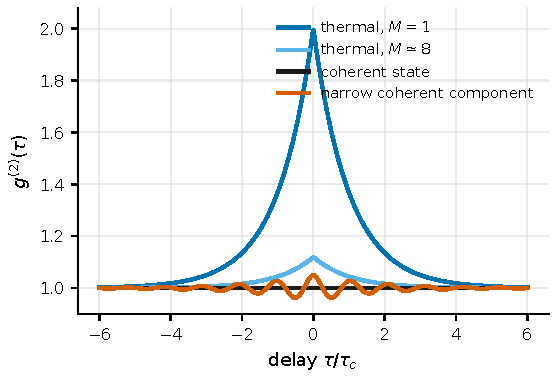
\includegraphics[width=0.82\linewidth]{figures/generated/chapter_09/ch09_radiation_g2_diagnostics.pdf}
\caption{不同光场的 \(g^{(2)}(\tau)\)。单模热光在零延迟给出高度为 2 的聚束峰；多模平均把峰值压低（式 \eqref{eq:e16-mode-dilution}）；理想相干态接近 1；窄相干谱线或受激成分可以在接近泊松的背景上留下小幅振荡或窄峰。横轴按相干时间 \(\tau_c\) 归一化。}
\label{fig:e16-g2-diagnostics}
\end{figure}

于是机制判断的正确姿势，是把所有能测的量收进同一个观测向量里联合诊断，而不是死盯平均谱：
\begin{equation}
  \bm{d}=
  \left\{
  I_\nu(t),\,
  Q_\nu(t),U_\nu(t),V_\nu(t),\,
  g^{(2)}_{ab}(\tau;\nu_i,\nu_j),\,
  \Delta t_{\rm var},\,
  \Omega_{\rm s}
  \right\}.
  \label{eq:e16-diagnostic-vector}
\end{equation}
\begin{formulaexplain}
\(\bm{d}\) 机制诊断观测向量；同时收集强度、Stokes 偏振、二阶相关、变异时标、角尺度。机制判断要靠这些量\emph{联合}约束，单看平均谱不够。
\end{formulaexplain}
其中 \(Q,U,V\) 是 Stokes 参数，下标 \(a,b\) 标记望远镜、偏振或频率通道，\(\Delta t_{\rm var}\) 是变异时标，\(\Omega_{\rm s}\) 是角尺度约束。把各机制放到这个向量里，指纹就分开了：热源——低偏振、有限 \(T_b\)、（稀释后残余的）热聚束；光薄同步——高线偏振、幂律谱；maser——窄线、极高 \(T_b\)、强偏振；FRB——极高 \(T_b\)、毫秒到微秒结构、色散、强偏振。而散射和等离子体传播会改变时间结构和频谱，却\emph{不该}被误当成源本身的发射统计。图 \ref{fig:e16-diagnostic-plane} 把其中两条轴（亮温、偏振分数，点大小示意可测二阶相干对比度）画成一张诊断平面，帮我们一眼定位一个源大致落在哪一类机制里。

\begin{figure}[tbp]
\centering
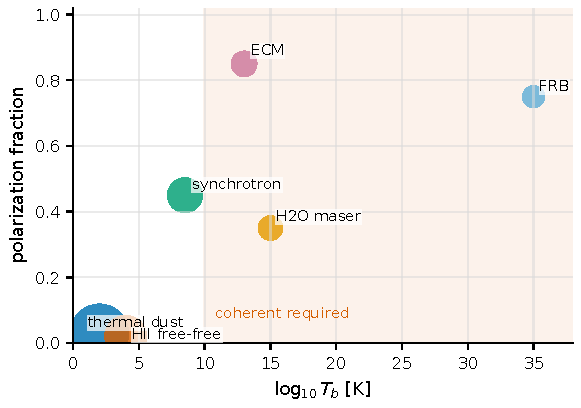
\includegraphics[width=0.86\linewidth]{figures/generated/chapter_09/ch09_diagnostic_plane.pdf}
\caption{辐射机制的联合诊断平面。横轴亮温，纵轴偏振分数，点大小表示可测二阶相干对比度的量级。热尘埃和 HII 区在低亮温低偏振区；同步辐射偏振较高但亮温通常低于相干爆发；electron-cyclotron maser、分子 maser 和 FRB 进入高亮温区，需要相干发射、泵浦或电荷成团来解释。}
\label{fig:e16-diagnostic-plane}
\end{figure}

\section{本章要点}
\label{sec:e16-summary}

\begin{itemize}
  \item \textbf{一句话主线。}把辐射机制翻译成"占有数 + 光子统计"：平均谱 \(I_\nu\) 只是一阶信息，光子到达相关（\(g^{(2)}\)）、偏振相关、跨频联合概率才是机制的指纹。
  \item \textbf{亮温就是占有数。}在 Rayleigh--Jeans 定义下 \(\bar n_\nu=k_BT_b/(h\nu)\) 精确成立（式 \eqref{eq:e16-occupation-from-tb}）。恒星可见光 \(\bar n_\nu\sim10^{-2}\)（稀薄），FRB \(\bar n_\nu\sim10^{36}\)（协同）。非相干射电亮温上限约 \(10^{9}\)--\(10^{10}~{\rm K}\)，超过就需相干机制。
  \item \textbf{热与非热都默认给混沌光。}只要"许多独立发射体相加、窄带内相位随机"，电场就是高斯过程，Siegert 关系给单模 \(g^{(2)}(0)=2\)（式 \eqref{eq:e16-siegert}）。黑体、自由自由、同步、逆康普顿——谱和偏振各异，光子统计同属混沌热光那一档。
  \item \textbf{只有相干机制可能偏离。}maser／激光靠粒子数反转和受激辐射，相干曲率辐射靠电荷成团（功率 \(\propto N^2\)）。它们打破"独立相加"前提，占有数和亮温冲破上限——但天体 maser 不等于实验室单模激光。
  \item \textbf{非经典光极难隔离。}模式稀释（式 \eqref{eq:e16-mode-dilution}）把 \(g^{(2)}_{\rm meas}(0)-1\sim1/M_{\rm eff}\) 压到 \(10^{-2}\) 甚至更低；候选机制本就稀少；仪器与传播效应还会伪造相关。机制判断必须用联合诊断向量 \eqref{eq:e16-diagnostic-vector}，并借第 \ref{chap:e13}、\ref{chap:e14} 章的排查工具对账。
\end{itemize}

\noindent\textbf{想一想。}(1) 一颗恒星的射电端和光学端，物质温度相同，为什么占有数 \(\bar n_\nu\) 差好几个量级？(2) 同步辐射谱是幂律、偏振可达 70\%，凭什么说它的光子统计和黑体属同一档？(3) 若你在数据里看到 \(g^{(2)}(0)=1.01\)，在下"探到聚束"的结论前，你至少要排除哪三类假信号？
